\section{Архитектура БД}

Спроектированная БД имеет следующий вид:

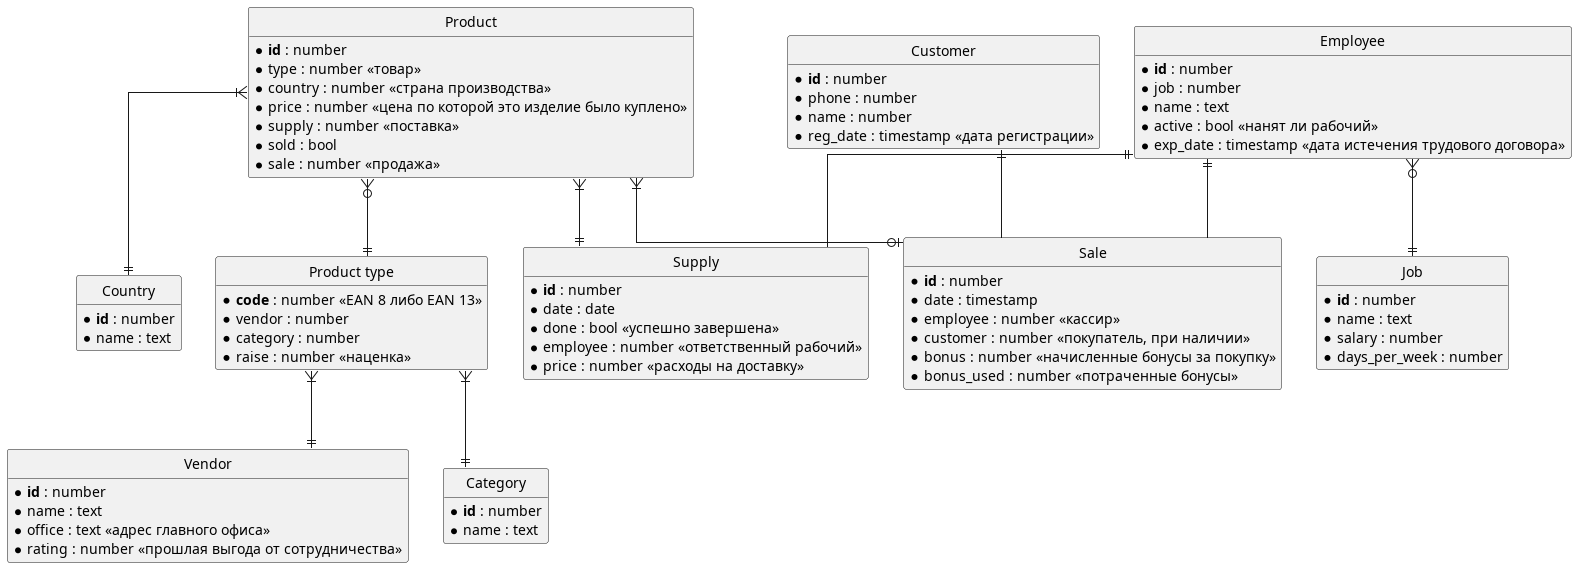
\includegraphics[width=16cm]{res/diagram.png}

\subsection{Товар}

Товар в бд представляется двумя сущностями. "Product" является конкретной товарной единицой. Он так же содержит базовую информацию о товаре, такую как цена закупки, айди поставки, продан ли он и если да, то ссылка на объект продажи и тд. "Product type" - тип товара, определяемый штрих-кодом.

Здесь следует немного отступить и объяснить зачем такое разделение и почему оно выполняется именно таким образом. Очевидно, что у каждого производителя есть как тип товара, так и конкретные единицы, которые поставляются. Тип товара регулируется на законодательном уровне при помощи выдачи государством штрих-кодов. Часть штрих-кода хранит информацию о производителе, часть о номере товара среди ассортимента производителя.

В пример можно привести производителя "каждый день". У него есть много канцелярских товаров, в том числе и ручек с различным форм-фактором. Даже если цвет у этих ручек будет один их штрих-коды будут отличатся, так как на законодательном уровне это разные товары. Это и есть тип товара. А конкретные единицы - конкретные ручки.

\subsection{Поставки и рабочие}

Для отслеживания поставок используется сущность "Supply". Она хранит все планируемые и проведенные поставки. Дополнительно о каждой из них хранится дата, расходы и ответственный сотрудник (человек от магазина, отвечающий за качество и количество прибывшего товара).

Информация о рабочих хранится в таблице "Employee". После увольнения рабочих из базы данных не удаляют. Это необходимо для того, что бы у старых поставок (и покупок), оставался ответственный сотрудник, даже если позже он будет уволен. Дополнительно хранится дата истечения трудового договора. Она полезна как в целом для понимания когда следует обновить контракт с текущим рабочим, так и для удаления слишком "старых" ответственных за поставки. 

Таблица "Job" хранит информацию о должности.

\subsection{Продажи и покупатели}

Все покупки хранятся в таблице "Sale". Здесь присутсвует ссылка на рабочего (кассира), дата, покупатель. Важно отметить, что баллы, начисляемые за покупку по программе лояльности хранятся здесь же. Это спорное решение, оно облегчает добавление новых записей (не нужно модифицировать "Customer"), но осложняет списание.

"Customer" хранит информацию о покупателе, которая может быть полезна при массовых рассылках.

\subsection{Связи и NF}

В первую очередь стоит отметить, что на рисунке \textbf{для всех сущностей} жирным обозначер основной ключ, который уникален для каждой записи и однозначно соответствует всем остальным записям.

У каждого "Product type" есть "Vendor" и "Category", так как все типы товаров имеют производителей и категорию, согласно которой они могут располагатся в магазине. При этом одна производитель/категория могут соответствать нескольким типам товара.

Товар ("Product"), обязательно имеет тип, страну производства (что можно вынести в тип товара, но не так важно) и поставку, в которой он был привезен в магазин. Так же, если товар продан, то он будет находиться в Sale.

Из соотношений один ко многим еще присутсвует отношение "Employee" и "Job", но здесь все просто. На одной вакансии могут работать несколько работников.